\section{Comparative Generative Quality}
\label{sec:comparative_generative_quality}

To systematically present our findings and provide a clear roadmap of the experiments, this chapter follows a structured progression:
\begin{itemize}
    \item \textbf{Model Selection (Section~\ref{subsec:model_selection}):} We evaluate paired (Pix2Pix) versus unpaired (CycleGAN) translation frameworks to identify the optimal architecture for Martian radar data.
    \item \textbf{Results of the GAN Comparison (Section~\ref{subsec:gan_comparison_results}):} We quantitatively and qualitatively benchmark the competing models using structural and perceptual metrics.
    \item \textbf{Sensitivity Analysis (Section~\ref{sec:sensitivity_analysis}):} We explore the impact of specific hyperparameters (e.g., patch size and loss weighting) on the generative quality.
    \item \textbf{Anomaly Detection Application (Section~\ref{sec:anomaly_detection_application}):} We deploy the optimal generator to isolate and detect subsurface anomalies.
\end{itemize}

\subsection{Model Selection Strategy}
\label{subsec:model_selection}

We began our experimental phase by selecting an appropriate generative architecture based on the relationship between the physical simulations and the observational data.
We initially evaluated Pix2Pix (previously detailed in Section~\ref{sec:modular_implementation}), a conditional GAN framework requiring paired image samples. 

We based this choice on the assumption that our physical approximations aligned spatially with the real radargrams.
We anticipated that the strong pixel-level supervision from the $L1$ regression loss would force the generator to directly superimpose realistic noise onto the simulations. 

However, empirical results revealed fundamental spatial misalignments, invalidating the paired assumption.
The Pix2Pix model rapidly overfit and generated high-frequency artifacts.
Instead of learning the SHARAD instrument's noise distribution, the network memorized specific training pairs.
The resulting images exhibited either excessive blurring (as the model averaged outcomes to minimize $L1$ error) or distinct checkerboard artifacts, failing to reproduce the stochastic clutter.

Consequently, we pivoted to the unpaired CycleGAN framework.
Simulated and real data share valid semantic content (subsurface stratigraphy) but lack strict pixel-to-pixel correspondence due to orbital positioning errors and simplified simulation physics. 

CycleGAN addresses this misalignment through the Cycle Consistency Loss, which enforces transitivity.
By requiring the round-trip translation ($A \rightarrow B \rightarrow A \approx A$) to match the original input, the model preserves structural information.
This mechanism allows the generator to adapt the surface clutter and add speckle noise without destroying the primary geological reflectors.
Only the genuine structural features survive the round-trip translation.

We highlight a critical trade-off: the balance between pixel-level accuracy and domain consistency.
Pix2Pix optimizes for numerical proximity rather than perceptual realism, making it unstable when processing imperfectly aligned scientific data.
CycleGAN relaxes the spatial constraint and prioritizes the statistical alignment of feature distributions.
We demonstrated that this domain-consistent approach is significantly more robust for SHARAD data.
CycleGAN generated sharper, more realistic textures and maintained the integrity of subsurface horizons.
These outputs proved highly suitable for downstream anomaly detection algorithms relying on structural coherence.


\subsection{Results of the GAN Comparison}
\label{subsec:gan_comparison_results}

We quantitatively and qualitatively compare the CycleGAN architecture with the Pix2Pix baseline.
We trained both models on the same dataset split and evaluated them on the test set using the metrics defined in Section~\ref{subsec:evaluation_metrics}.
We aim to understand how different training objectives affect the perceptual realism of the generated radargrams and their suitability for downstream anomaly detection.

\subsubsection{Quantitative and Qualitative Benchmarking}
Table~\ref{tab:benchmark_pix2pix_cyclegan} reports the average PSNR, SSIM, and LPIPS scores for both models.
Classical pixel-wise metrics (PSNR and SSIM) show similar results for Pix2Pix and CycleGAN, suggesting both networks reproduce the global structure of the radargrams at a coarse level.
We observe $PSNR_{\text{cyc}} \approx 23.0$~dB versus $PSNR_{\text{pix}} \approx 19.0$~dB, and comparable SSIM values.
Both models reconstruct large-scale stratigraphic interfaces and surface echoes with similar mean squared error and structural similarity.

\begin{table}[htbp]
    \centering
    \caption{Quantitative comparison between Pix2Pix and CycleGAN on the test set. The values are obtained from the benchmark script and correspond to mean scores over all test samples.}
    \label{tab:benchmark_pix2pix_cyclegan}
    \begin{tabular}{lcccc}
        \hline
        Model    & PSNR [dB] $\uparrow$ & SSIM $\uparrow$ & LPIPS $\downarrow$ & FID $\downarrow$ \\
        \hline
        Pix2Pix  & 19.0      & 0.234 & 0.254 & 11.03 \\
        CycleGAN & \textbf{23.0}      & \textbf{0.291} & \textbf{0.104} & \textbf{1.56} \\
        \hline
    \end{tabular}
\end{table}

However, the Learned Perceptual Image Patch Similarity (LPIPS) metric, introduced by Zhang et al.~\cite{Zhang_2018_CVPR}, reveals a pronounced difference.
The CycleGAN model attains a significantly lower LPIPS score ($0.104$) compared to Pix2Pix ($0.254$).
In the feature space of a deep convolutional network, CycleGAN outputs are perceptually closer to real SHARAD observations.
Figure~\ref{fig:lpips_distribution} illustrates these empirical distributions.

\begin{figure}[htbp]
    \centering
    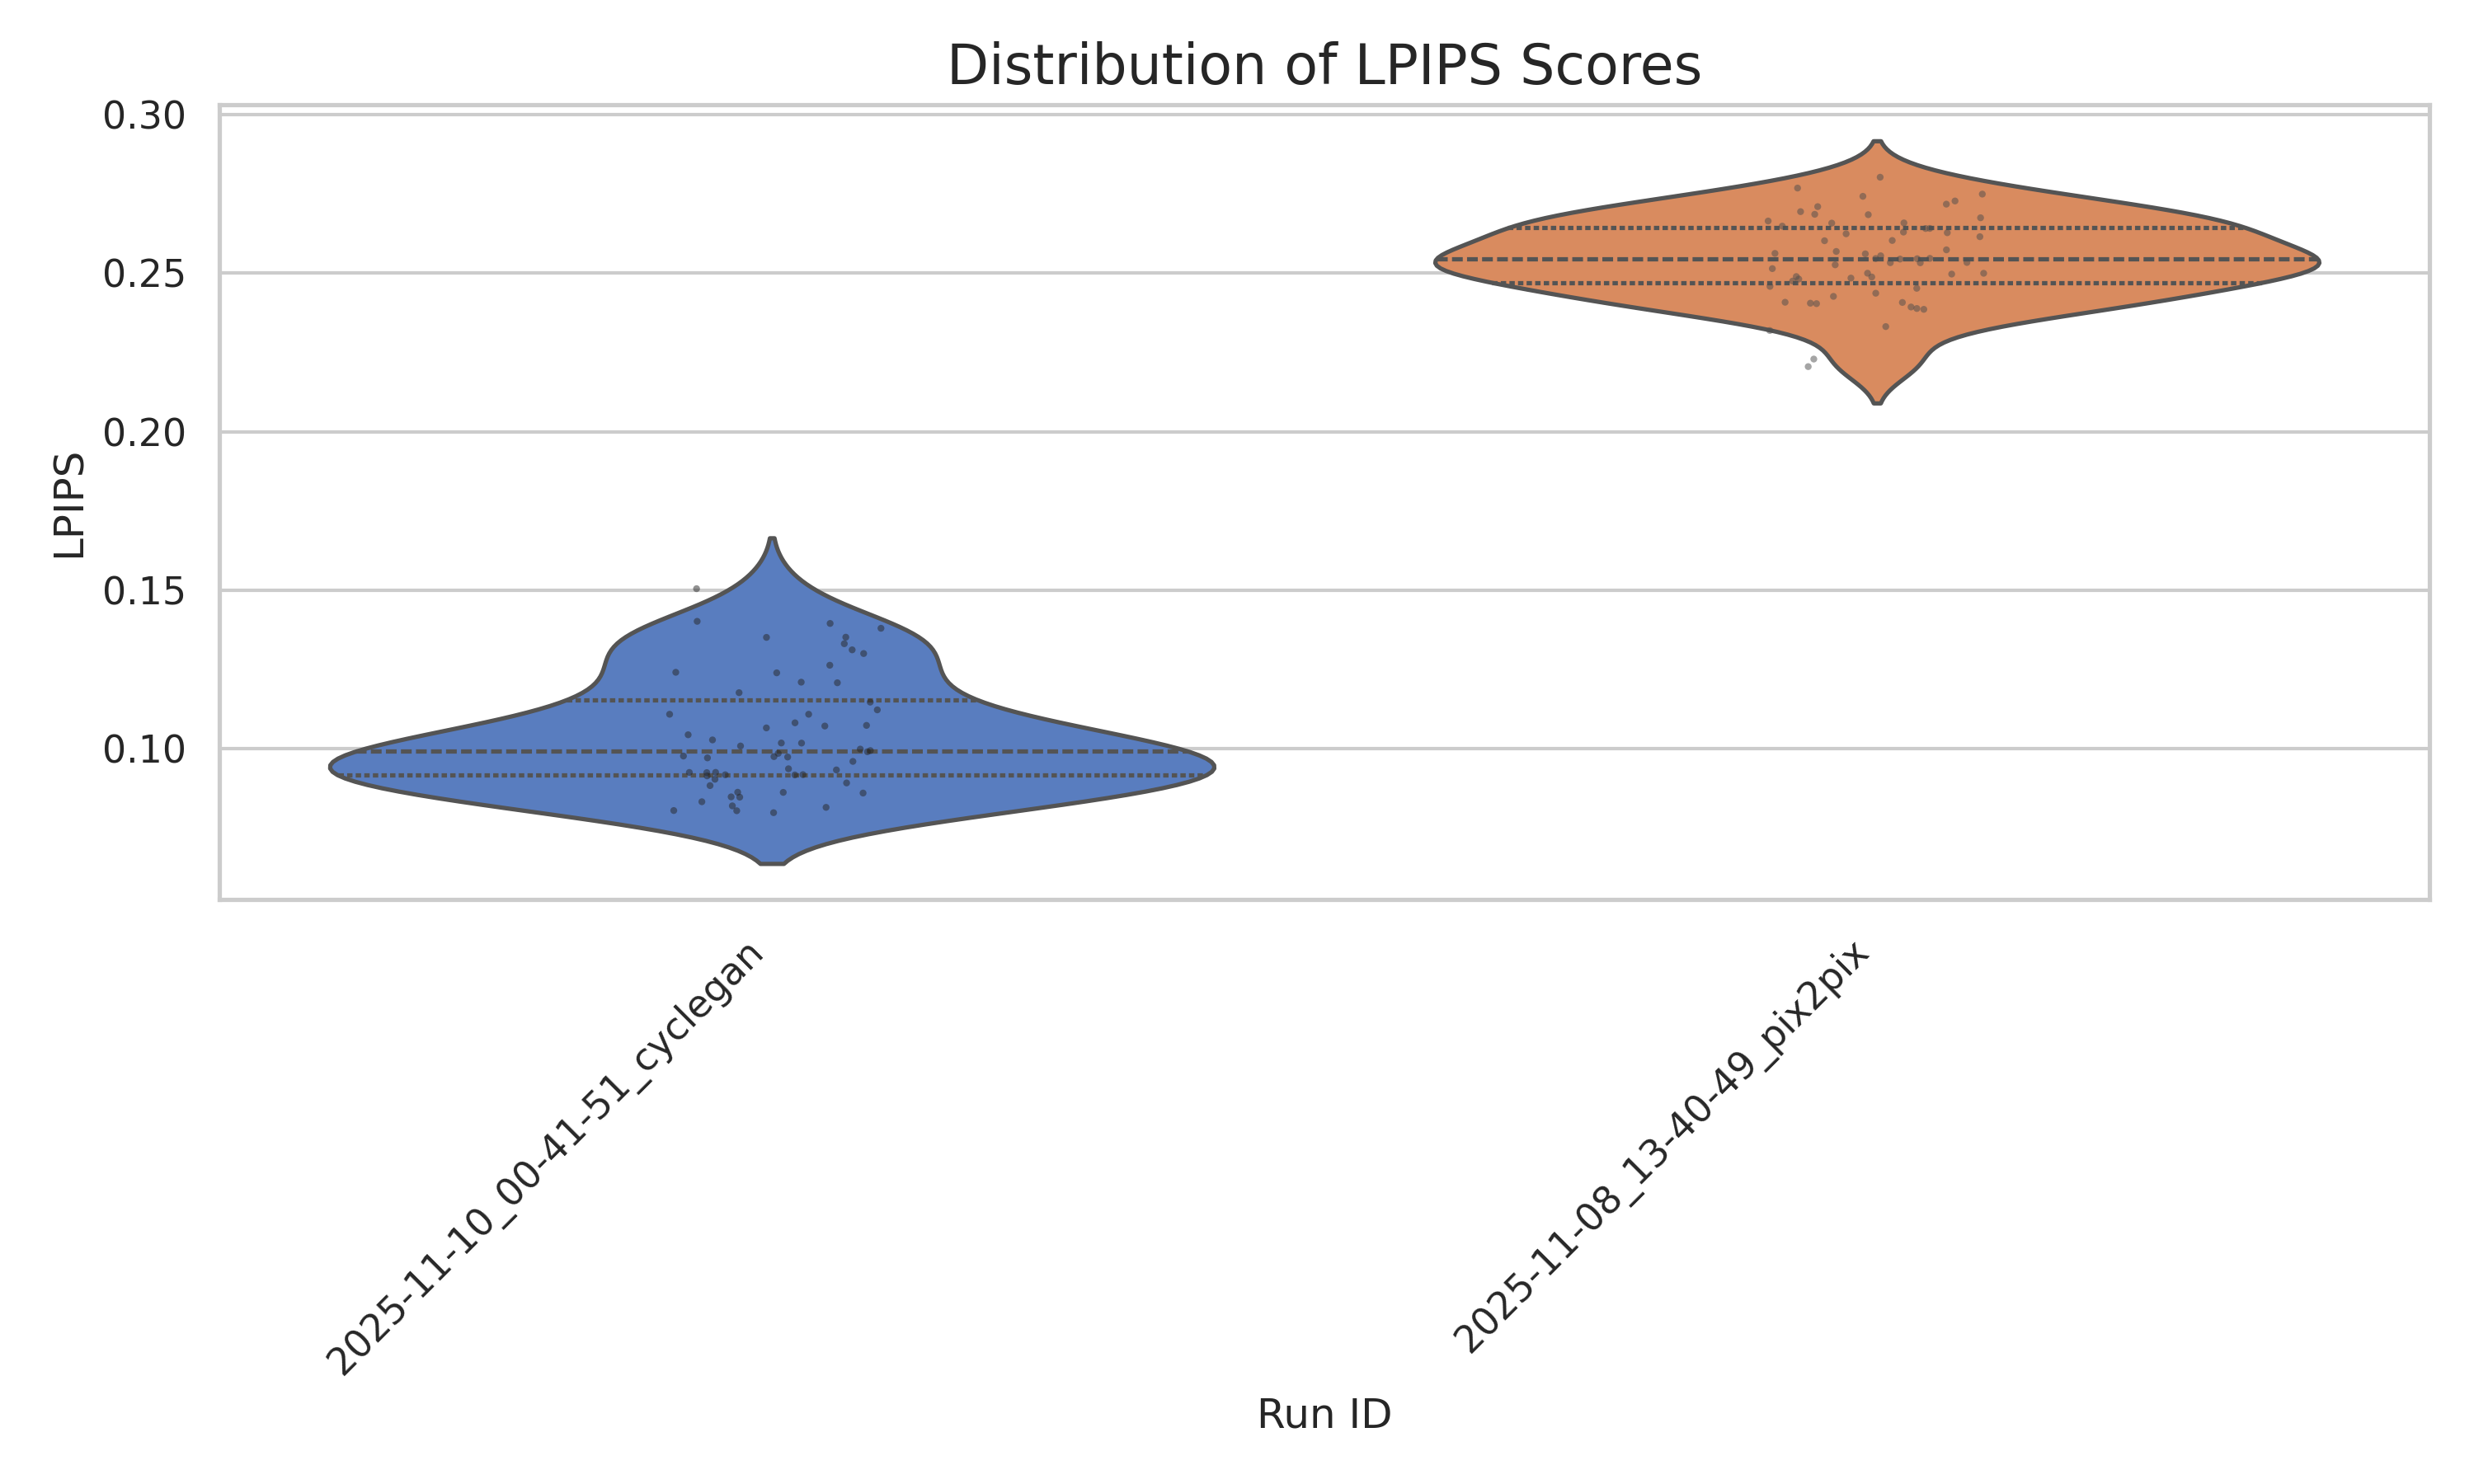
\includegraphics[width=0.6\textwidth]{images/benchmark/lpips_distribution.png}
    \caption{Distribution of the Learned Perceptual Image Patch Similarity (LPIPS) scores evaluated on the test set. The CycleGAN model exhibits a tightly clustered distribution with a significantly lower mean distance (0.104) compared to the wider, high-variance distribution of the Pix2Pix baseline (0.254). Lower values indicate generated textures that are perceptually closer to real Martian radargrams.}
    \label{fig:lpips_distribution}
\end{figure}

We confirm this interpretation through qualitative visual comparisons (see Figure~\ref{fig:qualitative_comparison}).
Driven by a strong L1 regression loss, Pix2Pix minimizes the average error by blending multiple plausible outcomes.
This mechanism causes excessive blurring and a loss of fine-scale texture.
The model blurs thin subsurface horizons and strongly attenuates the speckle pattern.
It yields images that are numerically close to the target but lack the characteristic \enquote{grain} of real radar data.

In contrast, CycleGAN leverages its adversarial loss and PatchGAN discriminator to match the local texture statistics of the real domain.
The objective function explicitly encourages the generator to synthesize realistic high-frequency speckle noise and small-scale clutter, tolerating minor pixel-level misalignments.
Consequently, the reconstructed radargrams preserve the \enquote{crispness} of the SHARAD signal. Hyperbolic diffractions, background noise, and subtle layering exhibit a granular appearance visually similar to real acquisitions.
This behavior directly benefits the subsequent anomaly detection pipeline.
It prevents artificial smoothness, which would otherwise generate spurious residuals and false positives when comparing real radargrams against synthetic baselines.

\begin{figure}[htbp]
    \centering
    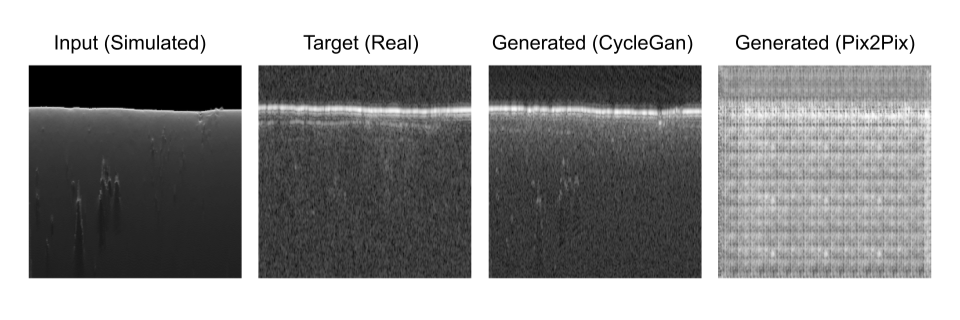
\includegraphics[width=\textwidth]{images/benchmark/comparison_sample_4}
    \caption{Qualitative comparison of Sim-to-Real translations. While the paired Pix2Pix model tends to average out structural details, leading to severe blurring artifacts and a loss of physical realism, the unpaired CycleGAN architecture preserves coherent stratigraphic horizons and synthesizes realistic high-frequency speckle noise characteristic of the real SHARAD domain. This visual behaviour is consistent with the significant gap in LPIPS and FID scores reported in Table~\ref{tab:benchmark_pix2pix_cyclegan}.}
    \label{fig:qualitative_comparison}
\end{figure}

\subsubsection{Feature Distribution Analysis}
To assess the generative consistency across diverse geological scenarios, we analyze the full probability density function of the scores rather than relying solely on dataset-wide averages.
As shown in Figure~\ref{fig:lpips_distribution}, we utilize \textbf{Violin Plots} to visualize these distributions.
The CycleGAN model exhibits a tightly clustered LPIPS distribution, indicating that it consistently produces high-quality textures across all tested patches.
In contrast, the Pix2Pix baseline shows a wider, high-variance distribution.
This visualization confirms that CycleGAN improves not just the average \textit{quality} of the generation, but also its \textit{reliability}, a critical requirement for scientific applications.

\subsubsection{Inference Efficiency and Reproducibility}
Beyond perceptual quality, we profiled the computational cost of the selected architectures.
We logged the inference time per patch during the benchmark loop to assess feasibility for planetary-scale processing.
For the deployed CycleGAN architecture ($128 \times 128$ patch input), the model achieves a mean inference latency of $\approx 4.2$~ms on an NVIDIA RTX 3090.
This performance confirms the system's viability for the real-time processing of massive orbital data streams.

Finally, to guarantee scientific rigor, the evaluation framework systematically versions all artifacts.
The system exports raw CSV metrics, high-resolution comparison grids, and summary JSON reports into timestamped output directories.
This ensures we can trace every experimental claim back to a specific, reproducible software execution context.

